%%%%%%%%%%%%%%%%%%%%%%%%%%%%%%%%%%%%%%%%%
% baposter Landscape Poster
% LaTeX Template
% Version 1.0 (11/06/13)
%
% baposter Class Created by:
% Brian Amberg (baposter@brian-amberg.de)
%
% This template has been downloaded from:
% http://www.LaTeXTemplates.com
%
% License:
% CC BY-NC-SA 3.0 (http://creativecommons.org/licenses/by-nc-sa/3.0/)
%
%%%%%%%%%%%%%%%%%%%%%%%%%%%%%%%%%%%%%%%%%

%----------------------------------------------------------------------------------------
%	PACKAGES AND OTHER DOCUMENT CONFIGURATIONS
%----------------------------------------------------------------------------------------

\documentclass[landscape,a0paper,fontscale=0.285]{baposter} % Adjust the font scale/size here
\usepackage[utf8]{vietnam}
\usepackage{graphicx} % Required for including images
\graphicspath{{figures/}} % Directory in which figures are stored

\usepackage{amsmath} % For typesetting math
\usepackage{amssymb} % Adds new symbols to be used in math mode

\usepackage{booktabs} % Top and bottom rules for tables
\usepackage{enumitem} % Used to reduce itemize/enumerate spacing
\usepackage{palatino} % Use the Palatino font
\usepackage[font=small,labelfont=bf]{caption} % Required for specifying captions to tables and figures

\usepackage{multicol} % Required for multiple columns
\setlength{\columnsep}{1.5em} % Slightly increase the space between columns
\setlength{\columnseprule}{0mm} % No horizontal rule between columns

\usepackage{tikz} % Required for flow chart
\usetikzlibrary{shapes,arrows} % Tikz libraries required for the flow chart in the template

\newcommand{\compresslist}{ % Define a command to reduce spacing within itemize/enumerate environments, this is used right after \begin{itemize} or \begin{enumerate}
\setlength{\itemsep}{1pt}
\setlength{\parskip}{0pt}
\setlength{\parsep}{0pt}
}

\definecolor{lightblue}{rgb}{0.145,0.6666,1} % Defines the color used for content box headers

\begin{document}

\begin{poster}
{
headerborder=closed, % Adds a border around the header of content boxes
colspacing=1em, % Column spacing
bgColorOne=white, % Background color for the gradient on the left side of the poster
bgColorTwo=white, % Background color for the gradient on the right side of the poster
borderColor=lightblue, % Border color
headerColorOne=black, % Background color for the header in the content boxes (left side)
headerColorTwo=lightblue, % Background color for the header in the content boxes (right side)
headerFontColor=white, % Text color for the header text in the content boxes
boxColorOne=white, % Background color of the content boxes
textborder=roundedleft, % Format of the border around content boxes, can be: none, bars, coils, triangles, rectangle, rounded, roundedsmall, roundedright or faded
eyecatcher=true, % Set to false for ignoring the left logo in the title and move the title left
headerheight=0.1\textheight, % Height of the header
headershape=roundedright, % Specify the rounded corner in the content box headers, can be: rectangle, small-rounded, roundedright, roundedleft or rounded
headerfont=\Large\bf\textsc, % Large, bold and sans serif font in the headers of content boxes
%textfont={\setlength{\parindent}{1.5em}}, % Uncomment for paragraph indentation
linewidth=2pt % Width of the border lines around content boxes
}
%----------------------------------------------------------------------------------------
%	TITLE SECTION 
%----------------------------------------------------------------------------------------
%
{
\includegraphics[height=4em]{logo.png}} % First university/lab logo on the left
{\bf\textsc{Nhận dạng khuôn mặt dùng thuật toán SIFT}\vspace{0.5em}} % Poster title
{\textsc{\{Bùi Thanh Tính, Nguyễn Văn Quảng, Nguyễn Việt Phú, Bùi Vũ Viết Phương, Nông Thành Nam\} 
\\
\hspace{12pt} Đại học Bách Khoa TP.HCM}} % Author names and institution
{
\includegraphics[height=4em]{logo.png}} % Second university/lab logo on the right

%----------------------------------------------------------------------------------------
%	OBJECTIVES
%----------------------------------------------------------------------------------------

\headerbox{Mục đích}{name=objectives,column=0,row=0}{

Nhóm đã tìm hiểu các bước cơ bản trong việc trích xuất và nhận dạng đặc trưng của thuật toán SIFT.

\begin{enumerate}\compresslist
\item Scale-space extrema detection
\item Keypoint localization
\item Orientation assignment
\item Keypoint descriptor
\end{enumerate}


\tikzstyle{decision} = [diamond, draw, fill=blue!20, text width=4.5em, text badly centered, node distance=2cm, inner sep=0pt]
\tikzstyle{block} = [rectangle, draw, fill=blue!20, text width=10em, text centered, rounded corners, minimum height=5em]
\tikzstyle{line} = [draw, -latex']
\tikzstyle{cloud} = [draw, ellipse, fill=red!20, node distance=3cm, minimum height=2em]

\begin{tikzpicture}[node distance = 2cm, auto]
\node [block] (init) {Scale-space extrema detection};
\node [cloud, left of=init] (Start) {Start};
\node [block, below of=init] (init2) {Keypoint localization};
\node [block, below of=init2] (init3) {Orientation assignment};
\node [block, below of=init3] (init4) {Keypoint descriptor};
\node [cloud, below of=init4] (End) {End};
\path [line] (init) -- (init2);
\path [line] (init2) -- (init3);
\path [line] (init3) -- (init4);
\path [line, dashed] (init4) -- (End);
\path [line, dashed] (Start) -- (init);
\end{tikzpicture}



\vspace{0.3em} % When there are two boxes, some whitespace may need to be added if the one on the right has more content
}

%----------------------------------------------------------------------------------------
%	INTRODUCTION
%----------------------------------------------------------------------------------------

\headerbox{Matching Keypoint}{name=introduction,column=1,row=0}{

Sau khi thực hiện bước trích xuất keypoint, ta phải so sánh các keypoint của ảnh gốc và ảnh input mục đích để nhận dạng.\\

\textbf{Input Image}: Là ảnh ta cần nhận dạng.\\

\textbf{Database}: Chứa các keypoint của ảnh trained.\\

\textbf{Threshold}: 15$\%$\\



\begin{center}
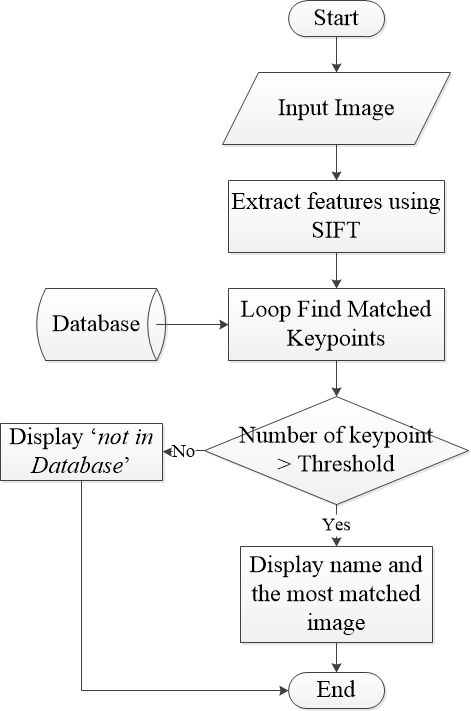
\includegraphics[width=1\linewidth]{thuatoan}
\captionof{figure}{Giải thuật nhận dạng}
\end{center}


}

%----------------------------------------------------------------------------------------
%	RESULTS 1
%----------------------------------------------------------------------------------------

\headerbox{Kết quả}{name=results,column=2,span=2,row=0}{


\begin{multicols}{2}
Khi có ảnh đầu vào (bên trái), hệ thống sẽ trích xuất keypoints rồi so sánh với keypoints ở trong database để nhận dạng.

\vspace{1em}
\begin{center}
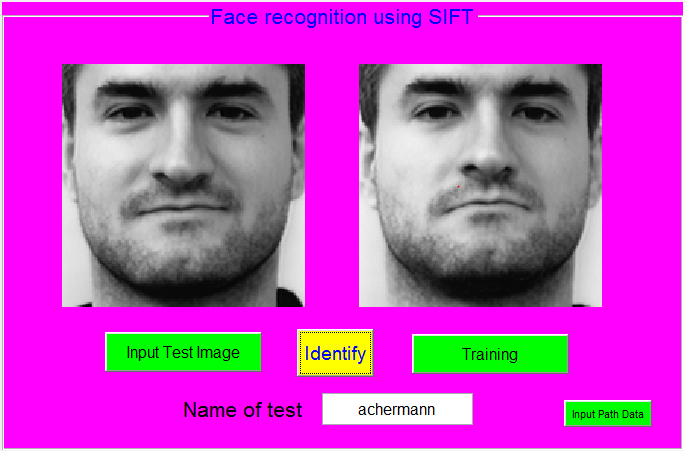
\includegraphics[width=1\linewidth]{ketqua1}
\captionof{figure}{Nhận dạng thành công}
\end{center}
\end{multicols}

%------------------------------------------------

\begin{multicols}{2}
\vspace{1em}
Nhưng khi dùng ảnh không có trong database thì nhận dạng thất bại.

\begin{center}
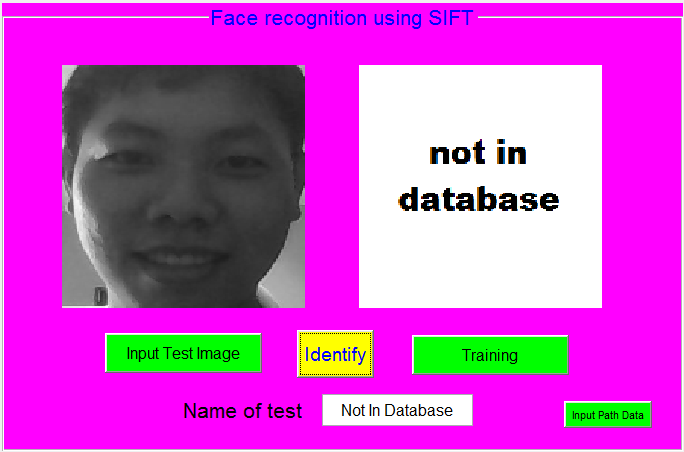
\includegraphics[width=1\linewidth]{ketqua2}
\captionof{figure}{Nhận dạng thất bại}
\end{center}

\end{multicols}
}

%----------------------------------------------------------------------------------------
%	REFERENCES
%----------------------------------------------------------------------------------------

\headerbox{Hướng phát triển}{name=references,column=0,above=bottom}{
Nhận dạng khuôn mặt \textbf{realtime}: Dùng thuật toán song song ($parallel$) chia nhỏ chương trình và thực hiện trên nhiều lõi CPU cùng lúc.

Nhận dạng vật thể.
}

%----------------------------------------------------------------------------------------
%	FUTURE RESEARCH
%----------------------------------------------------------------------------------------

\headerbox{Tài liệu tham khảo}{name=futureresearch,column=1,span=2,aligned=references,above=bottom}{ % This block is as tall as the references block

\begin{multicols}{2}
$[1]$  Lowe, D. 2004 \textit{"Distinctive image features from scale-invariant keypoints"}, International Journal of Computer Vision, Vol. 60, No. 2, 91–110.
\\
$[2]$ Brown, M. and Lowe, D.G. 2002.  \textit{"Invariant features from interest point groups"}.  In British Machine Vision Conference, Cardiff, Wales, pp. 656-665.


\end{multicols}
}

%----------------------------------------------------------------------------------------
%	CONTACT INFORMATION
%----------------------------------------------------------------------------------------

\headerbox{Thông tin liên lạc}{name=contact,column=3,aligned=references,above=bottom}{ % This block is as tall as the references block

\begin{description}\compresslist
\item[Nhóm 9] Môn học: Xử lý ảnh.
\item[Email] nhom9xulyanh@gmail.com
\item[Phone] 0973 816 840
\item[Github] https://github.com/nvquang97
\end{description}
}

%----------------------------------------------------------------------------------------
%	CONCLUSION
%----------------------------------------------------------------------------------------

\headerbox{Kết luận}{name=conclusion,column=2,span=2,row=0,below=results,above=references}{

\begin{multicols}{2}
\textbf{ƯU ĐIỂM}

Keypoint ít phụ thuộc vào:
\begin{enumerate}\compresslist
\item Cường độ sáng
\item Che khuất
\item Góc xoay
\item Méo dạng
\end{enumerate}

%------------------------------------------------
\textbf{NHƯỢC ĐIỂM}

SIFT có các nhược điểm sau:

\begin{enumerate}\compresslist
\item Khó nhận dạng nếu có nhiễu muối tiêu.
\item Thời gian nhận dạng không nhanh.
\item Tốn bộ nhớ chương trình.
\end{enumerate}


\end{multicols}

}
%----------------------------------------------------------------------------------------
%	MATERIALS AND METHODS
%----------------------------------------------------------------------------------------

\headerbox{phương pháp lập trình}{name=method,column=0,below=objectives,bottomaligned=conclusion}{ % This block's bottom aligns with the bottom of the conclusion block
Nhóm dựa vào code của \textbf{behindthesciences.com} để lập trình trên Matlab.\\
Ngoài ra nhóm đã lập trình GUI để người dùng dễ dàng tương tác hơn.
}



%----------------------------------------------------------------------------------------

\end{poster}

\end{document}